A multiscale simulation for the analysis of the mechanical behaviors of soft biological tissues was developed and implemented using AMSI. The biotissue simulation is currently a two-scale hierarchical multi-scale simulation coupling two continuum analyses. The primary scale (engineering scale) is a macro-scopic simulation using the finite element method on the cauchy momentum balance equation. The tertiary scale is micro-scopic and takes place at every macro-scale integration point (those points where the stress response of the material is queried during the macro-scale simulation) and used to supply the material response. The micro-scale simulation simply conducts a force-balance operation on a randomly generated collagen fiber-network residing inside of a unit cube representative volume element (RVE) which is deformed using the state of the associated macro-scale element, and has appropriate boundary conditions enforced. More detail into the derivation of this multi-scale system can be found in \cite{stylianopoulos2008thesis} \cite{agoram2001coupled} \cite{stylianopoulos2007multiscale} . Discussion of the dimensionalization of the dimensionless force terms (the upscaling operation from micro-scale to macro-scale) produced by each fiber network can be found in \cite{stylianopoulos2007volume} \cite{chandran2007deterministic}.

\begin{figure}
  \begin{center}
    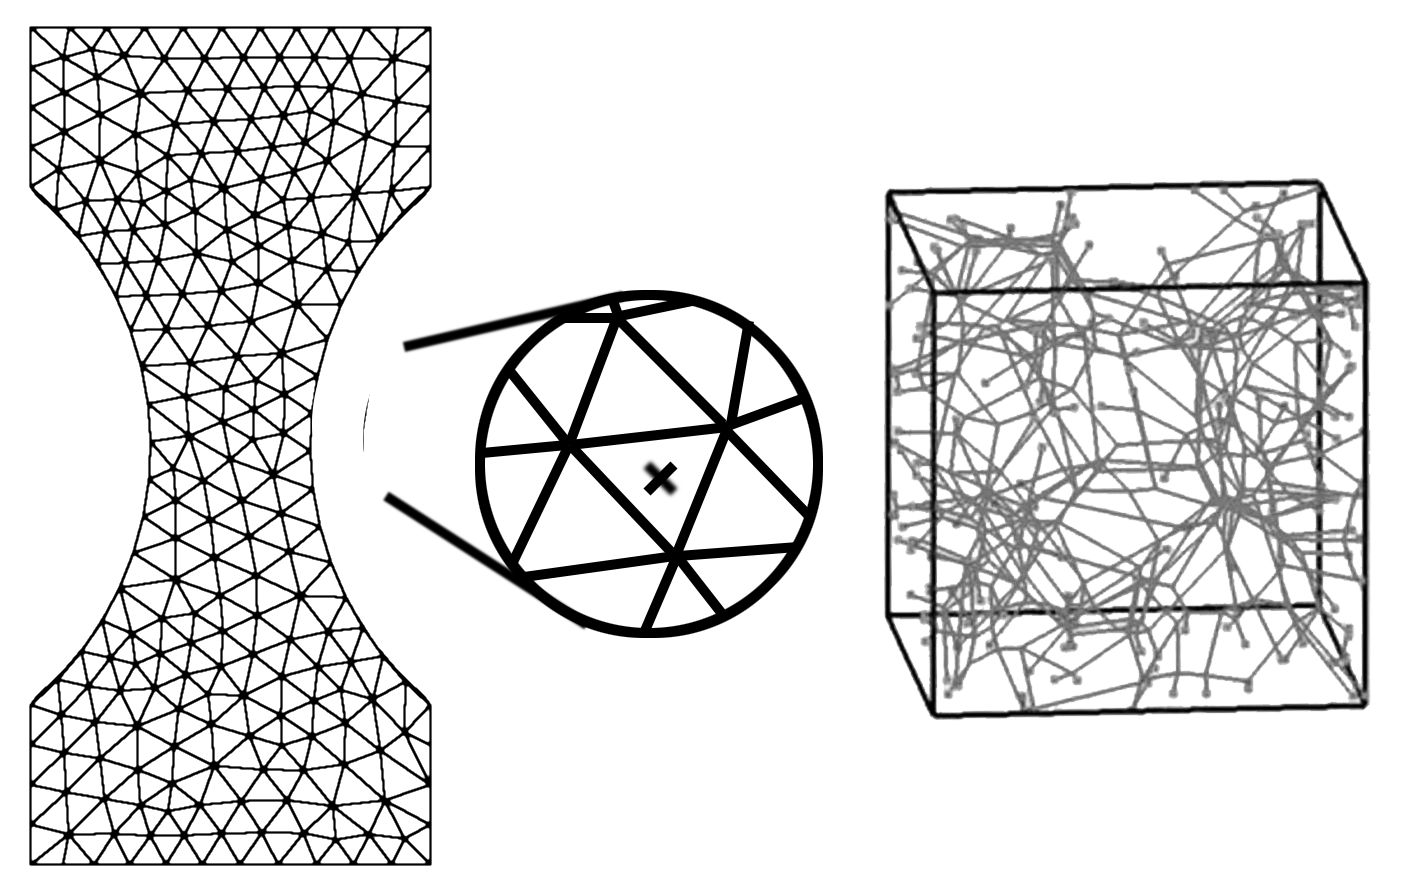
\includegraphics[height=3in]{biotissue-scales.png}
  \end{center}
  \caption{\small Biotissue multi-scale domains}
  \label{biotissue_scales}
\end{figure}

The biotissue simulation was implemented by combining two single-scale simulations: a typical parallelized finite element analysis and a quasistatics code. The combination of these two simulations using AMSI was very straightforward, involving the introduction of an initialization and configuration phase for AMSI, wrapping the pre-existing main functions of each simulation in an AMSI scale-task callback, and finally introducing relavant AMSI communcation (and load-balancing) calls at locations where scale-interaction is required. 

The simulation has been run many times on the Amos BlueGene/Q managed by the Center For Computational Innovations at Rennselaer Polytechnic Institute, and has scaled up to 250k elements at macro-scale with over 16k cores (over 90\% assigned to micro-scale simulations as these represent the bulk of actual computation). Scaling beyond this should be possible but has not currently been conducted. Theoretically the simulation should be able to scale up to around 300 million elements, limited by memory restrictions on the AMOS machine and the memory associated with a single RVE. Scaling to the full machine is however necessary to get a richer understanding of the performance of AMSI.

Symposia on the development and use of AMSI for the biotissue problem have been given at the SIAM Conference on Parallel Processing for Scientific Computing 2014 and at the SIAM Conference on Computational Science and Engineering 2015.

The Parallel Processing for Scientific Computing talk \cite{wtobin2014pp} was a discussion of the general layout and services provided by AMSI and the implementation of the biotissue example problem as well as initial performance results of the biotissue problem on a relatively modest (20k elements) mesh and a more reasonable mesh (200k elements).

\begin{figure}
  \begin{center}
    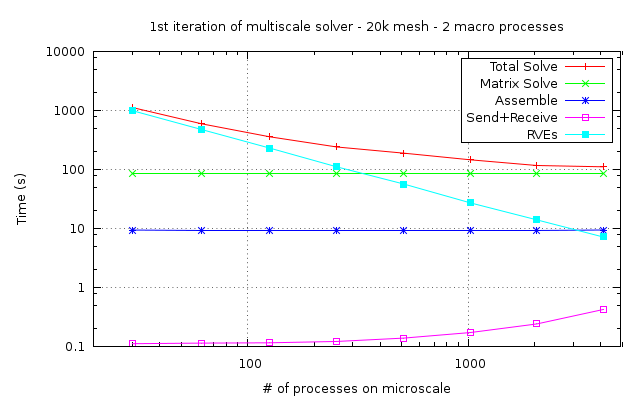
\includegraphics[height=3in]{allTimes_2macro_20k.png}
  \end{center}
  \caption{\small Multi-scale solver 1st iteration (20k elements)}
  \label{20k_first_iteration}
\end{figure}

Figure \ref{20k_first_iteration} is a weak scaling study conducted on a 20k element mesh, leaving the number of macro-scale processes constant and varying the number of micro-scale processes from just 32 to 8192 by powers of 2. The total time to assemble and solve a single tangent stiffness matrix at the engineering scale is considered (1 Newton-Raphson iteration), and different portions of the overall workload are shown. The actual matrix solve is unchanging as the number of macro-scale processes which compute the linear solve remains constant. Thus the matrix solve time represents the idealized optimal time to compute a single iteration. It is clear that as the number of micro-scale processes increases, the overall solve time approaches the matrix solve time, and while the communication time increases, it is still several orders of magnitude less than the overall solve time.

\begin{figure}
  \begin{center}
    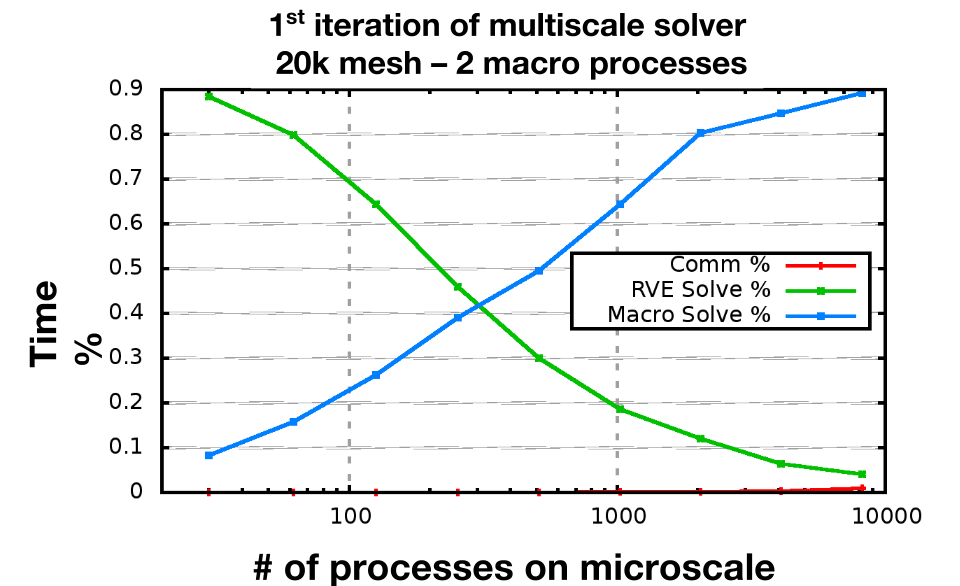
\includegraphics[height=3in]{siam_pp_weak_scaling.png}
  \end{center}
  \caption{\small Weak scaling on 20k mesh}
  \label{weak_scaling}
\end{figure}

Figure \ref{weak_scaling} is a view of the same weak-scaling study, weighted by the total time-to-solution for each case. Thus it is clear that as the number of micro-scale processes increase sufficiently, the overall computational load is dominated by the matrix solve. Increasing the number of processes at macro-scale should result in a reduction of this computational domincation, but both the size of macro- and micro-scales (and their ratio) must be considered when trying to determine the optimal allocation size. This figure suggests that a 1:128 macro-to-micro ratio will result in equal time being spent on both computations, and allow local load balancing operations at individual scales to make the most impact. Of course overall time-to-solution can be minimzed by simply allocating as many processes as possible, but allocating in the above ratio, weighted by the efficacy of individual scale load-balancing to impact the performance of a single scale, should result in the best possible gain. Further discussion and analysis of this concept will be published in \cite{wtobin2015mlb}.

\begin{figure}
  \begin{center}
    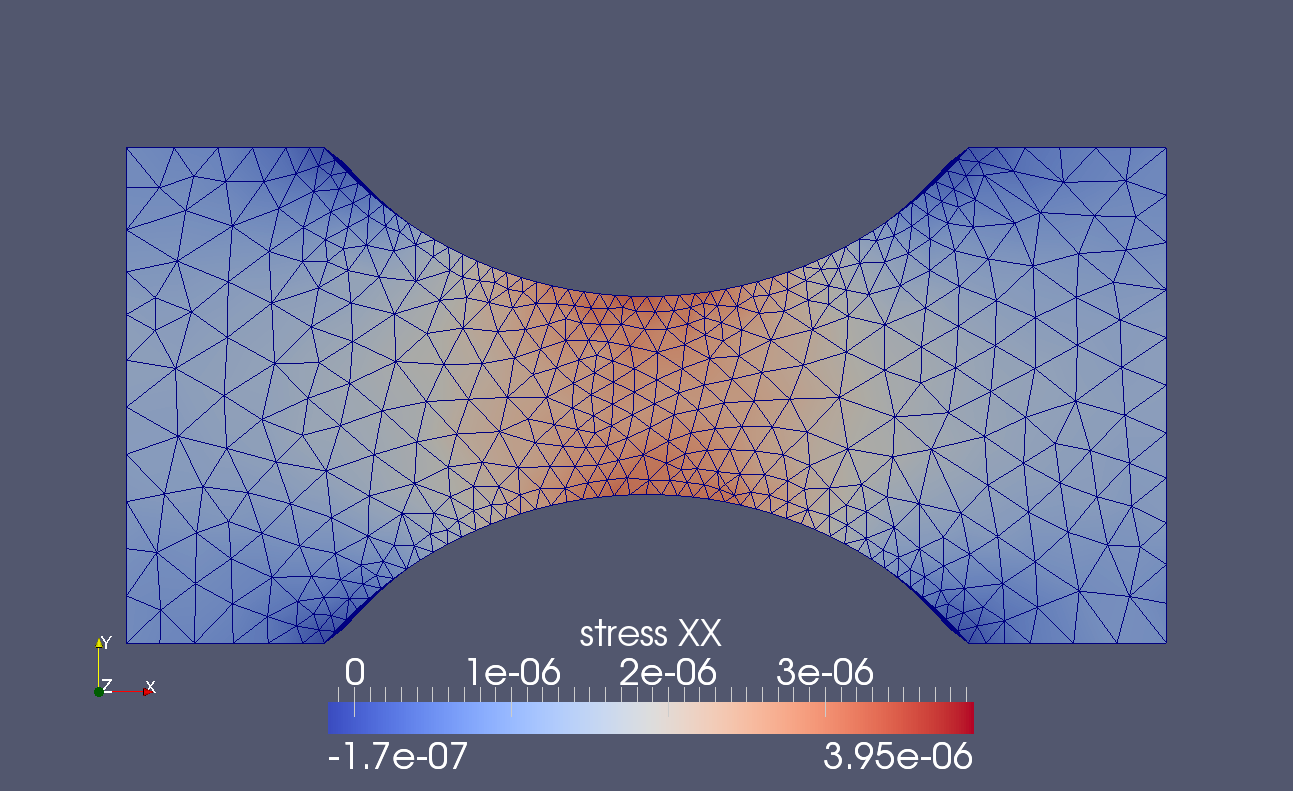
\includegraphics[height=3in]{dogBone14k.png}
  \end{center}
  \caption{\small Engineering scale mesh}
  \label{dogbone_mesh}
\end{figure}

The Computational Science and Engineering talk \cite{wtobin2015cse} was a discussion of the scale-sensitive load-balancing operations provided by AMSI and their usage in the Biotissue example problem. For this talk only the 20k mesh was used as the run times for a 200k mesh proved too long for a reliable turnaround on results, however the longer the computation (in terms of incremental load steps applied) the more benefit should be seen from the scale-sensitive load balancing. Longer runs on a larger (250k element) mesh are currently being conducted, as recent work on performance and memory footprint has allowed much quicker overall execuation times making larger runs feasible.

As each RVE is a nonlinear simulation their is no a-prior estimate of the computational load each RVE represents, so the optimal initial distribution is simply treating the weight of each RVE as 1. Thus each micro-scale process is assigned either $ \floor*{\frac{\text{num\_rves}}{\text{num\_micro\_procs}}} $ or $ \ceil*{\frac{\text{num\_rves}}{\text{num\_micro\_procs}}} $. Once the first load-balancing event is reached, regardless of the granularity at which load-balancing is occuring for a given case, each RVE has recorded the total number of newton iterations it has conducted since the previous load-balancing event. This number is used as a heuristic weighting metric to determine the computational load of each individual RVE. The iteration count metric was chosen as each iteration takes a similar level of work to complete, up to the difference in the number of RVEs for each unique fiber network. Further, assuming linear incremental loading, regions in the engineering-scale mesh located near stress concentrators will result in 'more interesting' boundary conditions for the micro-scale problems related to numerical integration points in that region, which may result in the RVE requiring more Newton iterations to converge to an adequate solution, since the boundary conditions may lie farther from the initial state of the RVE in the regime of convergence for the nonlinear problem.

\begin{figure}
  \begin{center}
    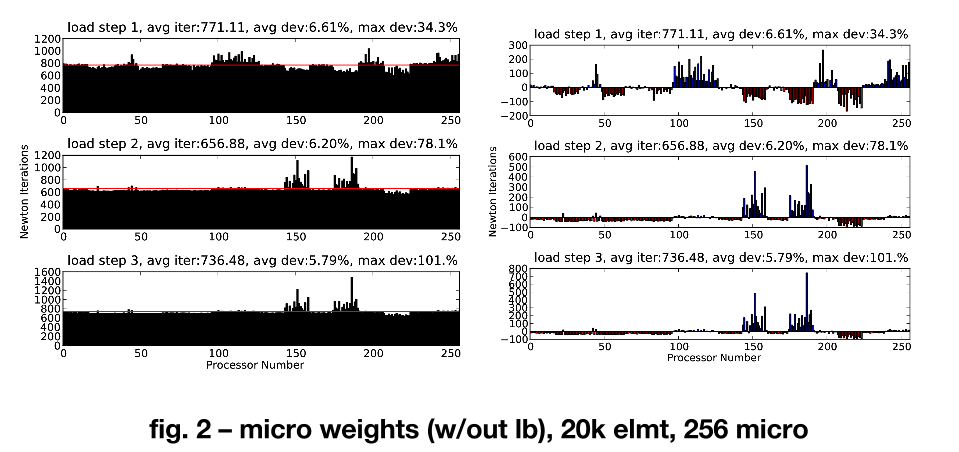
\includegraphics[height=2.5in]{siam_cse_initial.png}
  \end{center}
  \caption{\small Unbalanced load distribution (20k elements)}
  \label{initial_load}
\end{figure}

The initial distribution of weights is shown in figure \ref{initial_load}, with a 20k element macro-scale mesh and 256 processes assigned to compute micro-scale RVEs. The left graph shows the overall weight (the sum of all newton iterations for all RVEs assigned to a given process) while the right graph shows the deviation from the average. While the average deviation is under 10\% in all cases, the max deviation is what truly matters since all micro-scale RVEs must finish processesing before scale-coupling communication can take place and the macro-scale can continue to compute the elemental matrices and assemble a global tangent stiffness matrix. 

\begin{figure}
  \begin{center}
    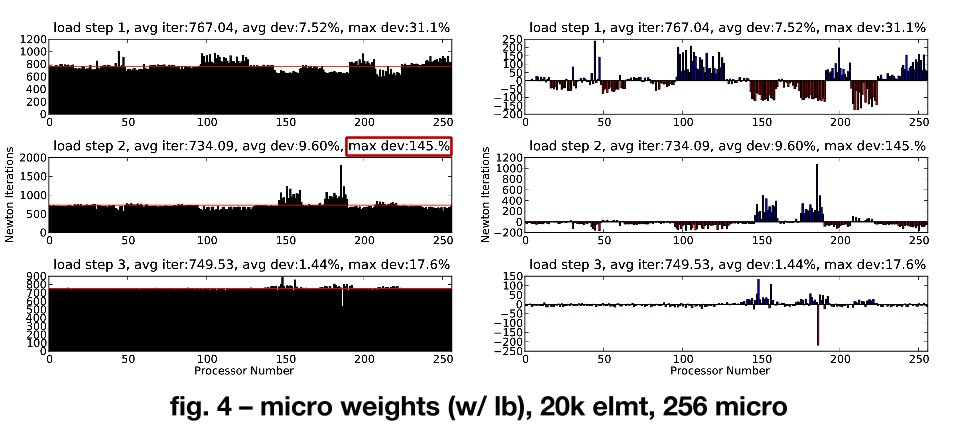
\includegraphics[height=2.5in]{siam_cse_updated.png}
  \end{center}
  \caption{\small Balanced load distribution (20k elements)}
  \label{load_balancing}
\end{figure}

Figure \ref{load_balancing} shows the result after scale-sensitive load-balancing (using the Zoltan libraries \cite{ZoltanOverviewArticle2002} \cite{ZoltanIsorropiaOverview2012} to plan the actual migration) is conducted. The maximal deviation after the first iteration is unfortunately much higher. But after that first iteration the max deviation is reduced by approximately 80\%. This is illustrative of the trend seen in the biotissue simulation, the number of micro-scale newton iterations conducted during the first incremental load step are not illustrative of the number of micro-scale newton iterations required during additional incremental load steps, which stay largely the same. Thus the first load balancing operation over corrects the issue, but the second and subsequent load-balancing operations result in better load balancing and run times overall. This can be seen more clearly in figure \ref{10_step_lb} which shows the weights for 64 micro-scale processes with the same mesh as above over 9 incrememental loading steps, the left graph shows the load without balancing and the right shows the load with balancing. The max deviation without load balancing stays in the 20\% range, while with load balancing it typically stays under 10\%, as low as 2.77\% in the 8th loading step.

\begin{figure}
  \begin{center}
    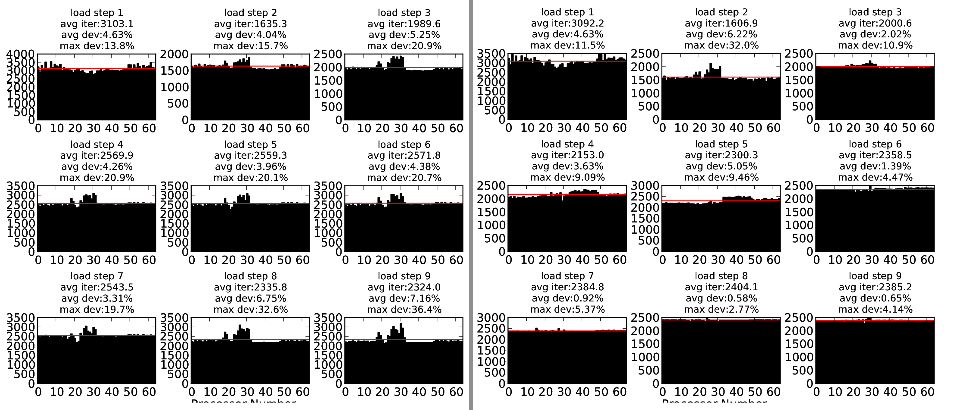
\includegraphics[height=3in]{siam_cse_ten.png}
  \end{center}
  \caption{\small Nine incremental loading steps (20k elements)}
  \label{10_step_lb}
\end{figure}
